\documentclass[a4paper,14pt]{extarticle}
\usepackage[utf8]{inputenc}
\usepackage[russian]{babel}
\usepackage{amsmath,amsfonts,amssymb}
\usepackage{geometry}
\usepackage{graphicx}
\usepackage{url}
\usepackage[nottoc, notlof, notlot]{tocbibind}
\usepackage{listings}
\usepackage{booktabs}

\geometry{top=2cm, bottom=2cm, left=3cm, right=1.5cm}
\lstset{
    inputencoding=utf8,
    extendedchars=\true,
    literate={-}{{-}}1 {\->}{{\texttt{->}}}2 {_}{{\_}}1,
    basicstyle=\ttfamily,
    frame=single,
    captionpos=b,
}

\begin{document}

\begin{titlepage}
    \begin{center}
        Санкт-Петербургский политехнический университет Петра Великого\\
        Физико-механический институт\\[4cm]
        
        \textbf{Отчёт по лабораторным работам 1 и 2}\\[0.5cm]
        по дисциплине «Интервальный анализ»\\[0.5cm]
        \textbf{«Калибровка чипа быстродействующей аналоговой памяти PCI DRS4»}\\[4cm]

        
        \begin{flushleft}
            Выполнил\\
            студент гр. 5040102/30201 \hfill Завьялов В.В. \hfill \rule{3cm}{0.1pt} \\[1.5cm]
            Проверил\\
            доцент, к.ф.-м.н. \hfill \hspace{1.9cm} Баженов А.Н. \hfill \rule{3cm}{0.1pt} \\[1.5cm]
        \end{flushleft}
        
        \vfill
        Санкт-Петербург\\
        2024 г.
    \end{center}
\end{titlepage}

\newpage

\tableofcontents

\newpage
\section{Постановка задачи}

Проводится исследование в области солнечной энергетики. Чип быстродействующей аналоговой памяти PCI DRS4 оснащён 8 каналами, каждый из которых содержит по 1024 ячейки. Каждая ячейка включает конденсаторы для хранения заряда и электронные ключи для записи сигналов и считывания напряжений через аналогово-цифровой преобразователь (АЦП). Ячейки объединяются в кольцевые буферы, обеспечивающие эффективное управление процессами записи и чтения данных.

При подаче сигнала синхронизации запись напряжений на конденсаторы прекращается, и фиксируется номер ячейки, в которую была сделана последняя запись. Основная задача данного исследования — калибровка данного чипа. Для этого в чип подаётся заранее известное напряжение $ X $, и считываются полученные значения $ Y $. Для каждого отдельного напряжения $ X $ операция повторяется 100 раз. Предполагается, что между $ X $ и $ Y $ существует линейная зависимость, и проводится определение коэффициентов регрессии $ \beta_0 $ и $ \beta_1 $.

\section{Теория}

\subsection{Первый подход: нахождение $\arg\max(\text{Tol})$}

Поскольку показания датчиков обладают погрешностью, полученные данные следует рассматривать не как точные значения, а как интервалы неопределённости. Центральное значение интервала совпадает с измеренным $ Y $, а радиус интервала равен:
$$
\epsilon = \frac{1}{16535}.
$$
Это отражает точность используемого АЦП. Поскольку показания с разных ячеек независимы, можно рассмотреть любую ячейку из всех 8192 (8 каналов по 1024 ячейки). Для выбранной ячейки имеется 100 пар значений $ (X, Y) $, где $ X $ находится в диапазоне $[-0.5, 0.5]$, а $ Y $ представлено интервалами с шириной $ \frac{2}{16535} $.

Для получения точечной оценки коэффициентов калибровки используется распознающий функционал $\text{Tol}$, который измеряет степень соответствия модели данным с учётом погрешностей:
$$
\text{Tol}(x, A, B) = \min_{1 \leq i \leq m} \left( \text{rad}(b_i) - \left| \text{mid}(b_i) - \sum_{j=1}^{n} a_{ij}x_j \right| \right),
$$
где:
\begin{itemize}
    \item $\text{rad}(b_i)$ — радиус интервала измерения $ Y_i $,
    \item $\text{mid}(b_i)$ — центральное значение интервала измерения $ Y_i $,
\end{itemize}

Матрица $ A $ и вектор $ b $ определяются следующим образом:
$$
A =
\begin{pmatrix}
x_0 & 1 \\
\vdots & \vdots \\
x_m & 1 \\
\end{pmatrix},
\quad
b =
\begin{pmatrix}
[y_0 - \epsilon, y_0 + \epsilon] \\
\vdots \\
[y_m - \epsilon, y_m + \epsilon] \\
\end{pmatrix}.
$$

Допусковое множество решений определяется как:
$$
\{ x \in \mathbb{R}^n \mid \text{Tol}(x, A, B) \geq 0 \}.
$$
Это означает, что модель полностью согласуется с измеренными данными с учётом погрешностей.

В случаях несовместимости системы уравнений необходимо увеличить радиусы интервалов измерений до тех пор, пока система не станет совместимой. Это достигается путём расширения интервалов $ Y $, что позволяет функционалу $\text{Tol}$ стать неотрицательным для всех измерений.

\textbf{Недостатки первого метода:}
\begin{itemize}
    \item \textit{Расширение интервалов:} При увеличении интервалов возникает значительная погрешность, так как интервалы растягиваются в обе стороны.
    \item \textit{Точечная оценка:} Первый метод предоставляет лишь точечную оценку коэффициентов $ \beta_0 $ и $ \beta_1 $, что может быть недостаточно информативно.
\end{itemize}

\subsection{Второй метод: нахождение оценки при помощи твинной арифметики}

Основные шаги метода:

\begin{enumerate}
    \item \textbf{Группировка данных:}
    \begin{itemize}
        \item Для каждого значения $ X $ собирается 100 значений $ Y $.
        \item Для каждой группы значений строится боксплот Тьюки, позволяющий определить внешние и внутренние оценки значений $ Y $.
    \end{itemize}
    
    \item \textbf{Построение интервалов:} На основе боксплотов формируются интервалы для $ Y $ для каждого $ X $. Каждому $ X_j $ соответствуют интервалы:
    $$
    Y_j = \left[ [y_{\text{in}, j}, y_{\text{in}, j}], [y_{\text{out}, j}, y_{\text{out}, j}] \right],
    $$
    где $ y_{\text{in}, j} $ и $ y_{\text{out}, j} $ — внутренние и внешние оценки значений $ Y $.
    
    \item \textbf{Распознающий функционал $\text{Tol}$:} Функционал $\text{Tol}$ создаётся на основе новых интервалов:
    $$
    \text{Tol}(x, A, B) = \min_{1 \leq i \leq m} \left( \text{rad}(b_i) - \left| \text{mid}(b_i) - \left( A \cdot x + B \right) \right| \right),
    $$
    где $\text{rad}(b_i)$ и $\text{mid}(b_i)$ определяют радиус и центральное значение интервала $ Y_i $, а $ A $ и $ B $ — текущие оценки коэффициентов.
    
    \item \textbf{Условия:}
    \begin{itemize}
        \item Если $\text{Tol}(\arg\max(\text{Tol})) = 0$, то найденные коэффициенты считаются оптимальными.
        \item Если $\text{Tol} > 0$, возвращается множество коэффициентов, удовлетворяющих этому условию.
        \item Если $\text{Tol} < 0$, соответствующие строки из матрицы $ A $ и вектора $ b $ исключаются, и процесс повторяется для достижения совместимости системы.
    \end{itemize}
\end{enumerate}

\section{Результаты}
В ходе эксперимента каждому датчику в чипе были присвоены соответствующие коэффициенты $B_0$ и $B_1$ в зависимости от его положения (координаты канала и ячейки).

Результаты для датчиков с координатами (2, 300) и (3, 300) изображены на рисунках 1-6.
\clearpage
\begin{figure}[htbp]
    \centering
    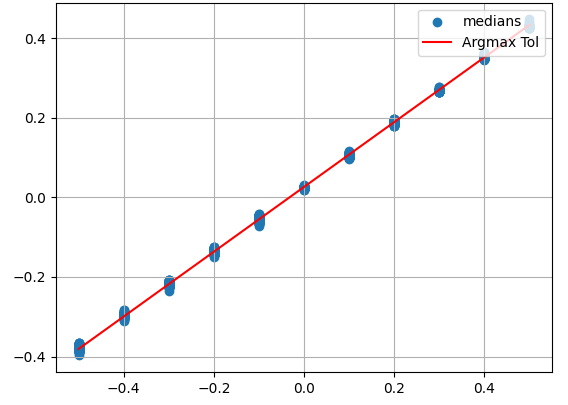
\includegraphics[width=0.6\textwidth]{f1.png}
    \caption{Регрессионная прямая для датчика (2, 300) полученная методом $\arg\max(\text{Tol})$}
    \label{fig:hamiltonianGraph}
\end{figure}

\begin{figure}[htbp]
    \centering
    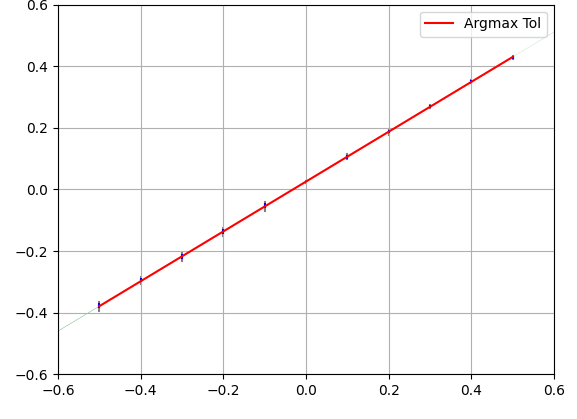
\includegraphics[width=0.6\textwidth]{f2.png}
    \caption{Регрессионная прямая для датчика (2, 300) полученная вторым методом}
    \label{fig:hamiltonianGraph}
\end{figure}
\clearpage
\begin{figure}[htbp]
    \centering
    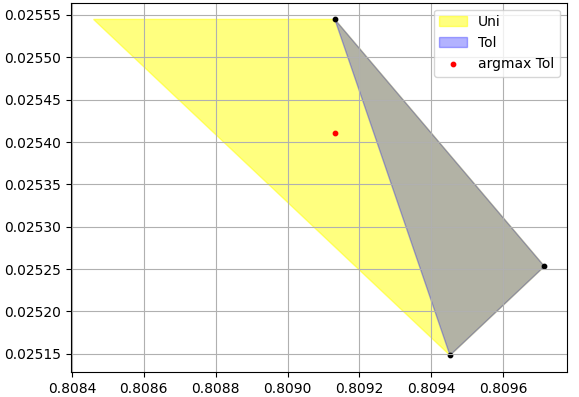
\includegraphics[width=0.6\textwidth]{f3.png}
    \caption{Tol, Uni и argmaxTol для датчика (2, 300)}
    \label{fig:hamiltonianGraph}
\end{figure}

\begin{figure}[htbp]
    \centering
    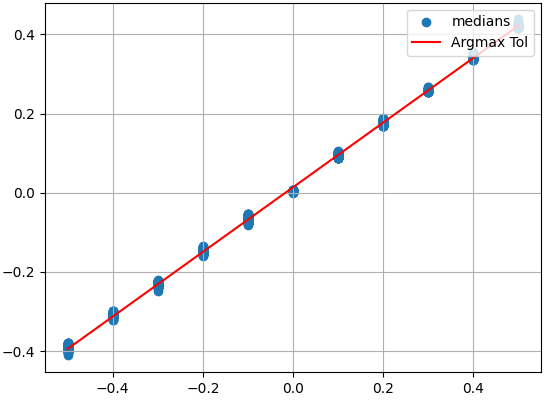
\includegraphics[width=0.6\textwidth]{f4.png}
    \caption{Регрессионная прямая для датчика (3, 300) полученная методом $\arg\max(\text{Tol})$}
    \label{fig:hamiltonianGraph}
\end{figure}
\clearpage
\begin{figure}[htbp]
    \centering
    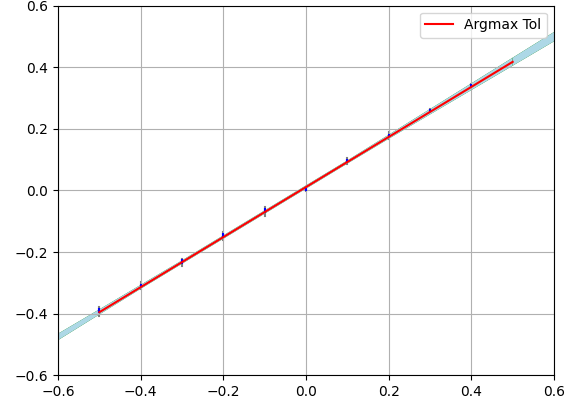
\includegraphics[width=0.6\textwidth]{f5.png}
    \caption{Регрессионная прямая для датчика (3, 300) полученная вторым методом}
    \label{fig:hamiltonianGraph}
\end{figure}

\begin{figure}[htbp]
    \centering
    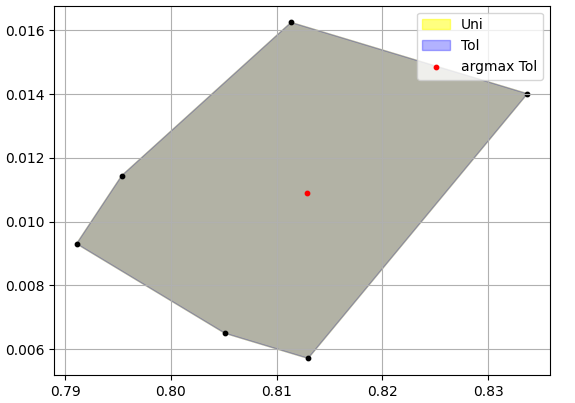
\includegraphics[width=0.6\textwidth]{f6.png}
    \caption{Tol, Uni и argmaxTol для датчика (3, 300)}
    \label{fig:hamiltonianGraph}
\end{figure}
\clearpage

\begin{table}[htbp]
    \centering
    \caption{Результаты}
    \label{tab:sensor_results}
    \small % Уменьшаем размер шрифта для таблицы
    \begin{tabular}{ccccc}
    \toprule
    \textbf{Координаты датчика} & \textbf{Метод} & \boldmath$\beta_0$ & \boldmath$\beta_1$ & \textbf{Кол-во модифицированных} \\
    \midrule
    (2, 300) & 1 & 0.814 & 0.026 & 1090 \\
    (2, 300) & 2 & 0.809 & 0.025 & 0 \\
    (3, 300) & 1 & 0.817 & 0.014 & 1093 \\
    (3, 300) & 2 & 0.813 & 0.011 & 30 \\
    \bottomrule
\end{tabular}
\end{table}

Анализ полученных графиков и итоговых данных подтвердил, что оба рассмотренных метода калибровки работают корректно. Несмотря на то, что их результаты во многом схожи, незначительные расхождения можно объяснить спецификой каждого из подходов:

\begin{itemize}
\item \textbf{Первый метод:} Позволяет оперативно получить точечные оценки коэффициентов, однако при расширении интервалов может вносить существенные погрешности.
\item \textbf{Второй метод:} Использование твинной арифметики и более тщательный подход к обработке данных обеспечивают более высокую точность результатов и устойчивость к выбросам.
\end{itemize}

Кроме того, замеченные различия в количестве выбросов между датчиками указывают на необходимость дополнительного анализа. Они могут быть связаны с техническими особенностями конкретных ячеек или каналов чипа.

\section*{Заключение}

В ходе лабораторной работы были изучены и реализованы два метода калибровки чипа PCI DRS4 с применением интервального анализа. По результатам видно, что оба метода демонстрируют схожие показатели. Кроме того, анализ показал, что по количеству модифицированных значений датчик с координатами (2, 300) имеет наименьшее количеством выбросов, тогда как датчик с координатами (3, 300) имеет наибольшее число выбросов.

\section{Код и ресурсы}
Репозиторий с кодом программы и кодом отчета:\\
https://github.com/Nochoooo/intervals

\end{document}